\chapter{РЕШЕНИЕ ЗАДАЧИ КЛАССИФИКАЦИИ}

В данной главе будут предложены несколько алгоритмов классификации вредоносных файлов, позволяющих с приемлемым качеством определять метку объектов, подготовленных нами ранее.
Действия в этой главе являются заключительными для создания классификатора. Мы будем использовать результат работы предыдущих глав, где мы создали необходимую выборку файлов, включающую в себя как вредоносные файлы, так и файлы, не причиняющие никакого вреда, а также собрали информацию о работе процесса “Microsoft Word”, специальным образом подготавливая каждый файл из выборки для запуска.

На практике очень часто методы машинного обучения тесно связаны с рассматриваемыми объектами и признаками, которые могут быть извлечены из них. Поэтому каждый предложенный нами алгоритм окажется отдельным подходом извлечения формального набора признаков для каждого исследуемого объекта. В зависимости от типа получившихся факторов мы будем использовать подходящий метод машинного обучения.

\section{Процесс как последовательность действий}

Для построения первой модели, мы рассмотрим процесс исполнения программы Microsoft Word, во время открытия каждого файла, как последовательность простых операций. В качестве операции будут выступать вызовы функций WinAPI, регистрируемые утилитой PROCMON, например такие как открытие файла, запись в файл или загрузка динамической библиотеки.

Во время создания того или иного набора признаков, принято обосновывать почему именно такой подход имеет право на жизнь. В нашем случае мы будем опираться на следующее предположение: последовательность действий, совершаемых вредосными файлами отличаются от нормального исполнения обычных пользовательских файлов. 

Имея на руках последовательность действий мы будем использовать технику, часто применяемую для построения различных языковых моделей натуральных языков. Только в отличии от традиционного использования таких методов, отдельным элементом языка у нас будет не слово на английском или русском языках, а операция, совершаемая запущенной программой. Каждый процесс в таком случае можно представить как документ, содержащий одно длинное предложение со словами из заданого множества.

Первый шаг необходимый для построения данной модели это перевод сырых данных, собранных с помощью утилиты PROCMON для каждого файла, в вектор слов. В нашем случае слово будет принадлежать конечному множеству операций, которые поддерживает PROCMON для перехвата, при этом мы будем рассматривать только подмножество операций непосредственно совершаемых Microsoft Word’ом и перехваченных во время исполнения.

\bgroup
\def\arraystretch{1.5}%  1 is the default, change whatever you need
\begin{table}[ht]
\caption{Пример операций и их отображений}
\label{tab_weight}
\centering
    \begin{tabular}{|c|c|}
    \hline \rowcolor{lightgray!50} Операция & Сокращённое обозначение \\
    \hline Process Start &  0 \\
    \hline Thread Create &  1 \\
    \hline QueryNameInformationFile &  2 \\
    \hline Load Image &  3 \\
    \hline CreateFile &  4 \\
    \hline
    \end{tabular}
\end{table}
\egroup

Для дальнейшей работы с этими операциями нам будет удобно отобразить их в короткие численные представления. Используя всё выше сказанное мы можем рассматривать элементы выборки как большие предложения, состоящие из чисел.

\bgroup
\def\arraystretch{1.5}%  1 is the default, change whatever you need
\begin{table}[ht]
\caption{Первые 10 операций, совершаемые запущенной программой, и их отображения}
\label{tab_weight}
\centering
    \begin{tabular}{|c|c|}
    \hline \rowcolor{lightgray!50} Операция & Отображение \\
    \hline Process Start &  0 \\
    \hline Thread Create &  1 \\
    \hline QueryNameInformationFile &  2 \\
    \hline Load Image &  3 \\
    \hline Load Image &  3 \\
    \hline CreateFile &  4 \\
    \hline QueryDeviceInformationVolume &  5 \\
    \hline QueryOpen &  6 \\
    \hline Load Image &  3 \\
    \hline CreateFile &  4 \\
    \hline
    \end{tabular}
\end{table}
\egroup

Например, если допустить что Таблица 4.2 содержит результат работы программы Microsoft Word от начала до конца, то объект, сгенерировавший данные операции, будет иметь вид: \textbf{“0 1 2 3 3 4 5 6 3 4”}.

Один из случаев, которые мы сможем определить такой моделью, является вызов некоторой аномальной функции, совершающей потенциально зловредные действия. Тогда слово, соответствующее отображению этой функции в число, не будет принадлежать никакому предложению, составленному по безвредным объектам. В таком сценарии мы можем использовать распределение частот по каждому слову, состоящему из цифр, для принятия решения. Однако, в некоторых случаях для нас может представлять опасность не только отдельный вызов функций, а некоторая последовательность вызовов безобидных подпрограм. Например, последовательность функций “CreateFile”, “ReadFile”, “WriteFile” может служить сигналом о создании копии вируса в системе. Чтобы учесть такие ситуации, мы будем использовать распределение N-грамм как обобщение частот отдельных слов. 

N-граммы для N равного 1 представляют из себя частоты каждого слова документа в отдельности. Для $N$ равного 2 это распределение пар слов и т.д. Например, рассмотрим такое распределение для объекта из Таблицы 4.2, где $N$ принимает значения из множества $\{1,2\}$.

\bgroup
\def\arraystretch{1.5}%  1 is the default, change whatever you need
\begin{table}[ht]
\caption{Разложение объекта из Таблицы 4.2 на $N$-граммы для \\ $N \in \{1, 2\}$}
\label{tab_weight}
\centering
    \begin{tabular}{|c|c|c|c|c|c|c|c|c|c|c|c|c|c|c|c|}
    \hline \rowcolor{lightgray!50} Тип N-граммы & 0 & 1 & 2 & 3 & 4 & 5 & 6 & 0 1 & 1 2 & 2 3 & 3 3 & 3 4 & 4 5 & 5 6 & 6 3 \\
    \hline Частота & 1 & 1 & 1 & 3 & 2 & 1 & 1 & 1 & 1 & 1 & 1 & 2 & 1 & 1 & 1 \\
    \hline
    \end{tabular}
\end{table}
\egroup

Количество различных N-грамм, конечно, зависит от самого значения числа N, поэтому его нужно выбирать из соображений баланса между длиной потенциально вредоносной последовательности и размером конечной матрицы объект-признак.
В нашем случае для создания рабочего метода мы будем использовать N равное 2, так как при установке $N = 1$ мы не будем учитывать связь между соседними действиями, а уже при $N = 2$ производится достаточное количество признаков для правильной классификации.
Последующее увеличение длины N соответственно не приводит к изменению качества в лучшую сторону.

Таким способом мы переведём каждый объект в вектор частот, получив в итоге матрицу объект-признак.
Как и в примере с объектом из таблицы 4.3, в качестве признака будет частота определённой N-граммы встретившейся в каждом объекте из обучающей выборки.

Это и дальнейшие преобразования будут производиться с помощью библиотеки Scikit-Learn для языка Python. ( Подробней про эти библиотеки и про язык ).

\bgroup
\def\arraystretch{1.5}%  1 is the default, change whatever you need
\begin{table}[ht]
\caption{Фрагмент матрицы объект-признак для двух хороших $\{G_0, G_1\}$ и двух плохих $\{B_0, B_1\}$ файлов.}
\label{tab_weight}
\centering
    \begin{tabular}{|c|c|c|c|c|c|c|c|c|c|c|c|c|c|c|c|c|c|c|c|c|}
    \hline & \multicolumn{20}{c|}{Различные виды $N$-грамм} \\
    \hline $G_0$ & 38 & 5 & 91 & 17 & 10 & 2 & 4 & 1 & 1 & 1 & 1 & 1 & 2 & 0 & 0 & 0 & 0 & 0 & 0 & 0 \\
 	\hline $G_1$ & 49 & 5 & 16 & 17 & 10 & 2 & 5 & 1 & 1 & 1 & 1 & 1 & 2 & 2 & 4 & 0 & 0 & 0 & 0 & 0 \\
 	\hline $B_0$ & 285 & 9 & 78 & 85 & 79 & 3 & 15 & 5 & 1 & 1 & 3 & 3 & 0 & 7 & 12 & 1 & 3 & 1 & 5 & 1 \\
 	\hline $B_1$ & 288 & 8 & 81 & 85 & 79 & 2 & 8 & 1 & 1 & 1 & 3 & 3 & 0 & 4 & 12 & 1 & 0 & 0 & 2 & 0 \\
	\hline
    \end{tabular}
\end{table}
\egroup

Имея на руках данную матрицу, мы можем воспользоваться ранее описаной линейной моделью. После обучения метода и проверки качества классификации с помощью подсчёта ошибок техникой LOO, мы заметим что метод со 100 процентным качеством определяет вредоносные файлы. То есть составленная нами выборка линейно разделима по какому-то набору признаков. Мы можем найти примеры таких признаков.

\bgroup
\def\arraystretch{1.5}%  1 is the default, change whatever you need
\begin{table}[ht]
\caption{Фрагмент матрицы объект-признак для двух хороших $\{G_0, G_1\}$ и двух плохих $\{B_0, B_1\}$ файлов.}
\label{tab_weight}
\centering
    \begin{tabular}{|c|c|c|}
    \hline Вид файла & QueryAllInformationFile, FileSystemControl \\
    \hline $G_0$ & 0 \\
 	\hline $G_1$ & 0 \\
 	\hline $B_0$ & 2 \\
 	\hline $B_1$ & 2 \\
	\hline
    \end{tabular}
\end{table}
\egroup

Нашу выборку можно разделить по последовательностям действий представленным в таблице 4.5.
Для нас это означает что существует последовательность операций, совершаемых только вредоносными объектами.
Разделяющие последовательности действий, найденые в исходных данных, продемонстрированны на рисунке 4.1.

\begin{figure}[ht]
    \centering
    \begin{subfigure}[h]{0.6\textwidth}
    \centering
        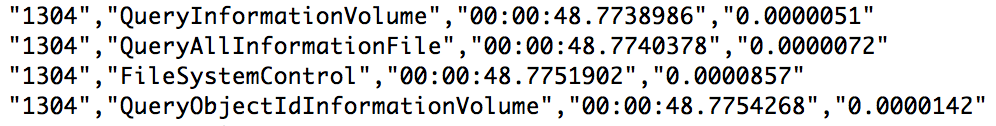
\includegraphics[scale=0.7]{pattern_0.png}
        \caption{}
        \vspace*{5mm}
    \end{subfigure}
    \begin{subfigure}[h]{0.6\textwidth}
    \centering
        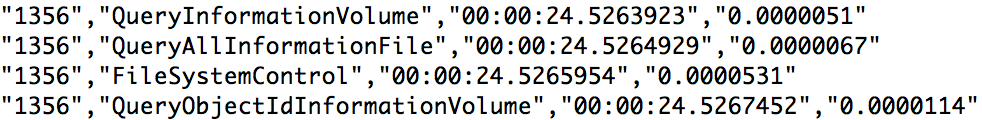
\includegraphics[scale=0.7]{pattern_1.png}
        \caption{}
    \end{subfigure}
    \caption{Разделяющие паттерны}
    \label{fig_parsetree}
\end{figure}

Не смотря на идеальную точность, данный результат считается недостаточно полным без дальнешего анализа происхождения данных операций, но подробный разбор работы Microsoft Word в случаях эксплуатаций различных уязвимостей является достаточно крупной задачей, достойной рассмотрения в отдельной работе.
Мы же ограничимся получившимся результатом, как первичной грубой оценкой при первичном анализе зловредных объектов.
Следующий метод основан на более сложном подходе, требующий объединения нескольких алгоритмов машинного обучения.

\section{Процесс как набор графиков}

В предыдущем параграфе был рассмотрен подход, основанный на разбиении выполнения процесса на простые операции с последующим анализом сгенерированных последовательностей операций.

Ранее нами был описан общий план проникновения и исполнения зловредного кода через эксплуатацию уязвимостей в сложных форматах файлов. Одним из этапов заражения является подготовка атакуемой программы для запуска шелл-кода. Часто в этот момент программа начинает вести себя необычно: зависать, работать медленней или аварийно завершаться. Чтобы отлавливать подобные ситуации автоматически, нам необходимо ввести набор формальных признаков, способных различать такие ситуации. Однако мы не можем подстраиваться под определённый вид поведения, например, завершение программы, потому что новый вирус, способный избегать появление такого демаскирующего признака, ускользнёт из нашего исследования.

В качестве обобщённого набора признаков, не привязанных к определённому виду визуального проявления, мы будем рассматривать время исполнения каждой операции. Время как признак является довольно чувствительными показателем работы процесса, если процесс будет вести себя необычно, то это прямо скажется на численных показателях времени. Исходя из таких рассуждений, был разработан новый метод извлечения формальных признаков работы из запущенной программы, основанный на представлении работы процесса в виде двумерного графика, где по оси X мы будем отображать номер операции, а по оси Y затраченное время на выполнение этой операции. 

То есть теперь в качестве признака выступает график, а не одно число, как в случае с частотой N-грамм. Это более богатое семейство, в отличии от N-грамм составленных по последовательностям из простых операций.

\begin{figure}[ht]
	\centering
    \begin{subfigure}[b]{1\textwidth}
    \centering
        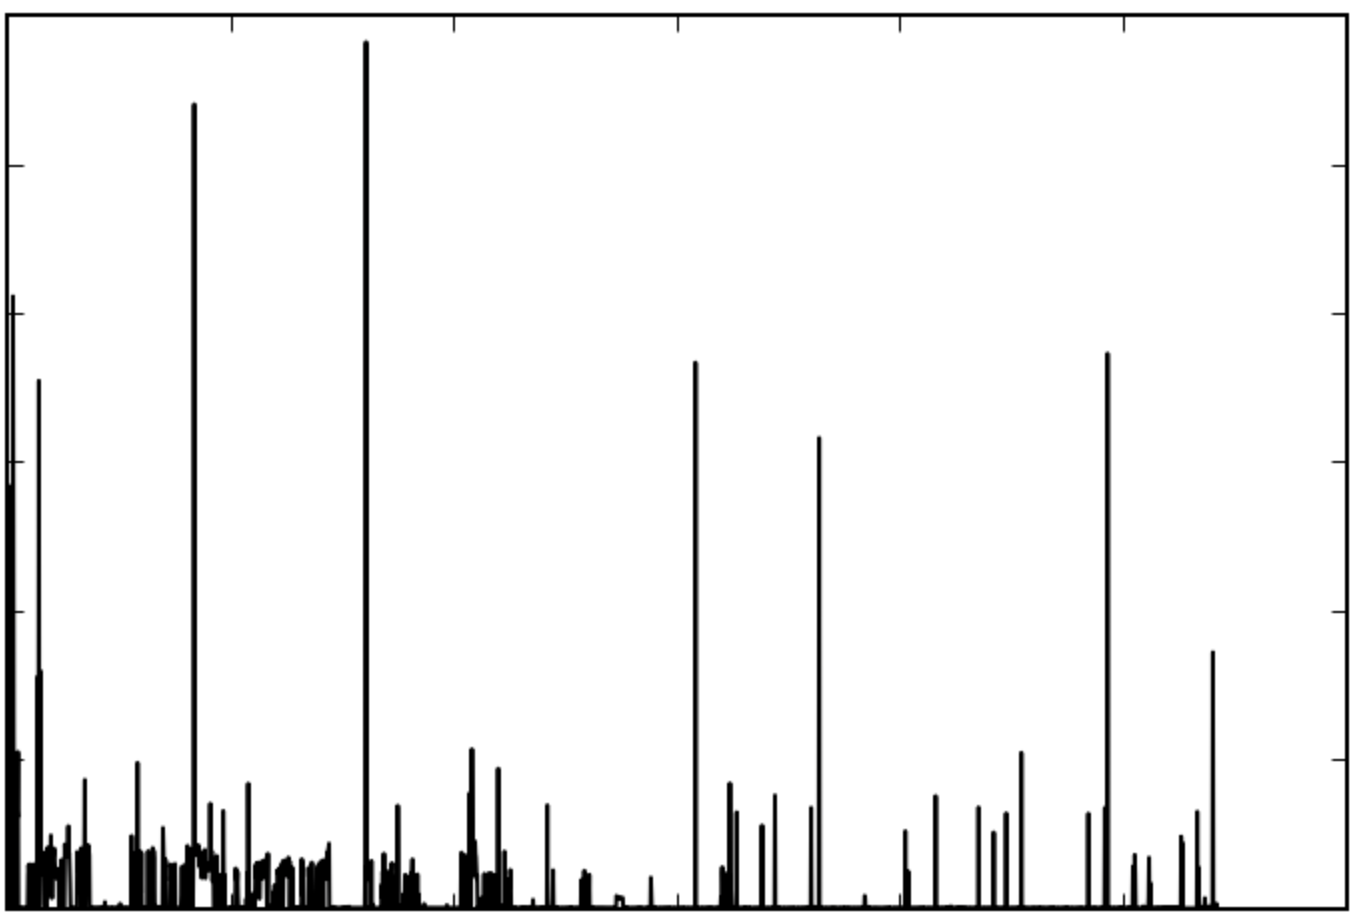
\includegraphics[scale=0.5]{pasted-image-29.png}
    \end{subfigure}
 
    \caption{График длительностей выполнения всех операций в течении работы одного из процессов Microsoft Word}
    \label{fig_parsetree}
\end{figure}

В графике, изображённом на Рисунке 4.1, по оси X были отображены операции всех типов в порядке их перехвата утилитой PROCMON. При работе больших программ вроде Microsoft Word многие операции производятся асинхронно, это означает что порядок некоторых групп операций неопределён. Как способ борьбы с этой проблемой мы можем разделить большой график, включающий все операций, на множество графиков, отображающих каждый тип операции в отдельности. Работа с множеством графиков также позволяет использовать некоторое подмножество операции, дающих наибольший прирост к качеству классификации. Подробности реализации такого отбора, будут рассмотрены в дальнейших параграфах.

\begin{figure}[ht]
	\centering
    \begin{subfigure}[b]{0.40\textwidth}
    \centering
        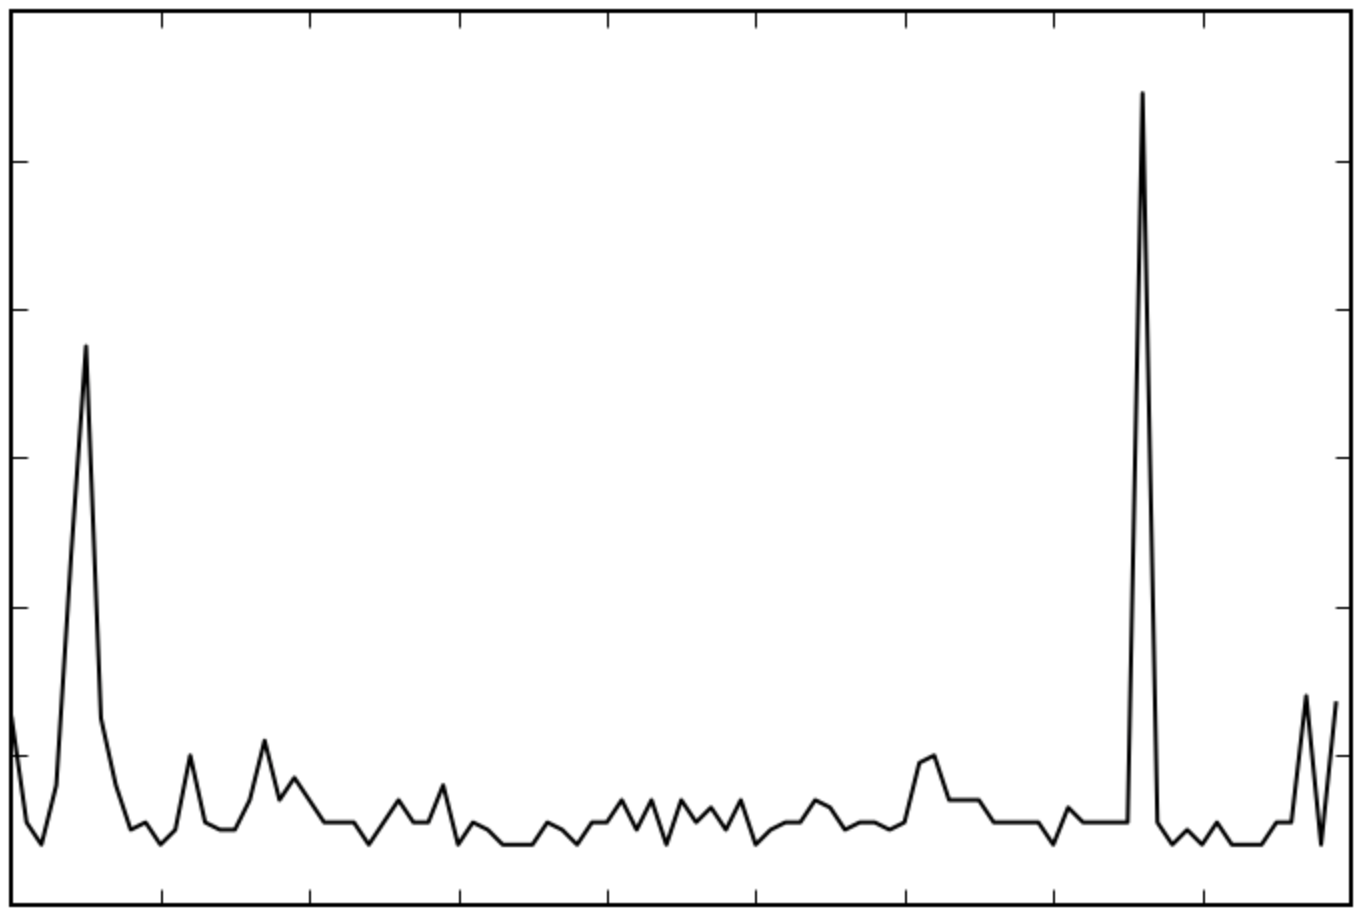
\includegraphics[scale=0.25]{pasted-image-31.png}
        \caption{}
    \end{subfigure}
 	\begin{subfigure}[b]{0.40\textwidth}
    \centering
        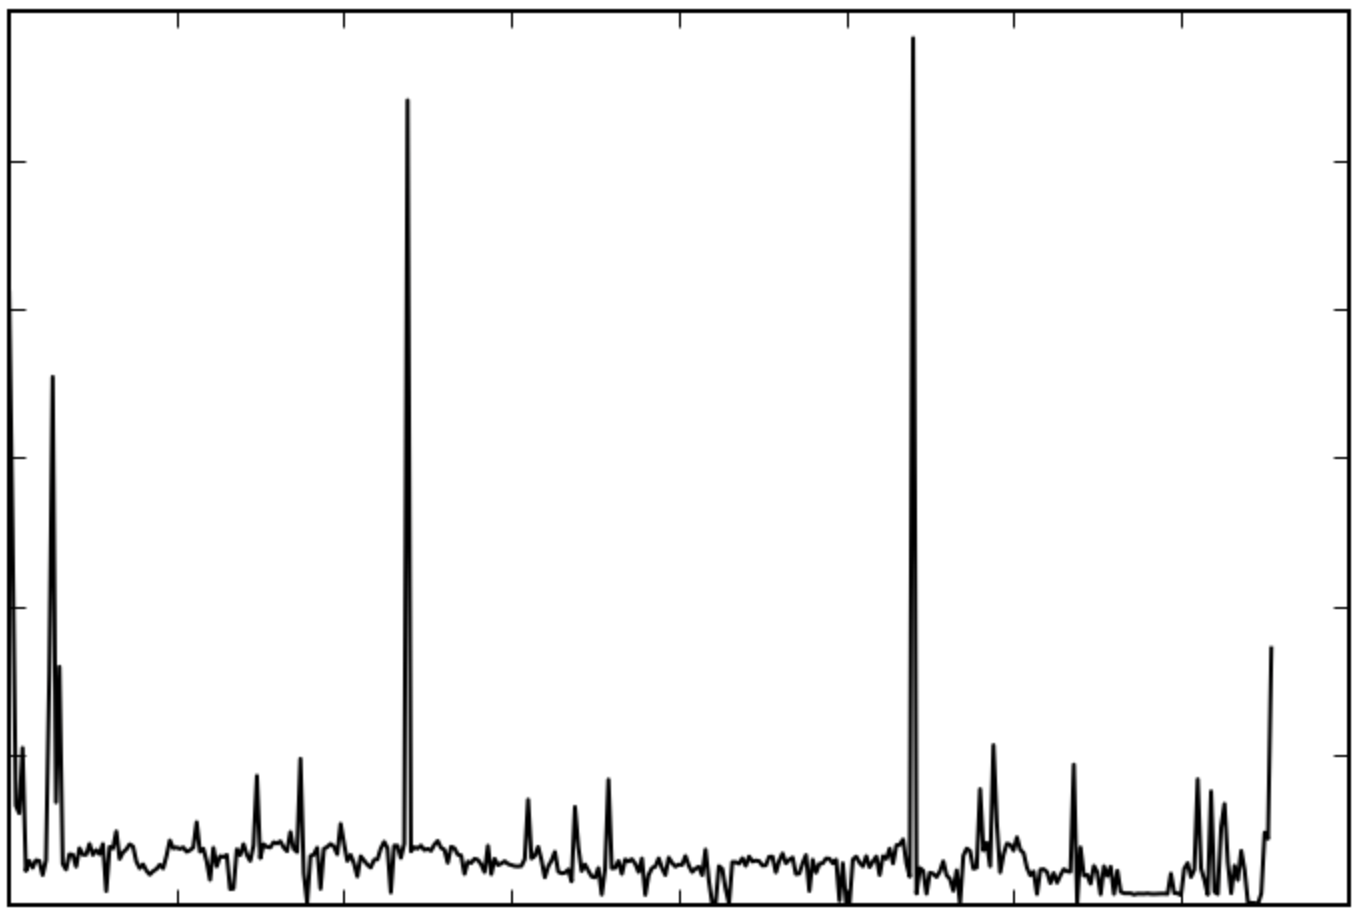
\includegraphics[scale=0.25]{pasted-image-33.png}
        \caption{}
    \end{subfigure}
    \caption{Графики операций (a) QueryBasicInformationFile и (б) ReadFile}
    \label{fig_parsetree}
\end{figure}

Итак мы разделили общий поток операций на несколько и, если в предыдущем параграфе в качестве признака объекта использовалась частота определённой N-граммы, то сейчас мы имеем набор графиков в качестве множества признаков. В отличии от действительных чисел, новые признаки в виде графиков не подходят для прямого использования в линейной модели и нам необходимо использовать другие методы машинного обучения. В данном случае, для решения задачи классификации, мы введём функцию расстояния между двумя сигналами и далее воспользуемся метрическим алгоритмом K ближайших соседей. Данную функцию мы будем использовать для каждого типа графиков в отдельности, поэтому при таком решении у нас возникнет вектор расстояний. Как мы увидим в дальнейшем, используя данный вектор, мы создадим целый набор классификаторов, после чего решим проблему их объединения.

\section{Функция расстояния между сигналами, алгоритм DTW}

Ранее получив набор графиков в качестве признаков объекта, нам понадобился алгоритм сравнения двух функций на близость. Человек, глядя на изображение нескольких функций, почти всегда сможет сказать похожи они или нет. В качестве простого примера можно рассмотреть набор из трёх графиков на рисунке 4.3. Довольно легко увидеть что графики B и C более схожи по значениям, чем графики A и C.

\begin{figure}[ht]
	\centering
    \begin{subfigure}[b]{1\textwidth}
    \centering
        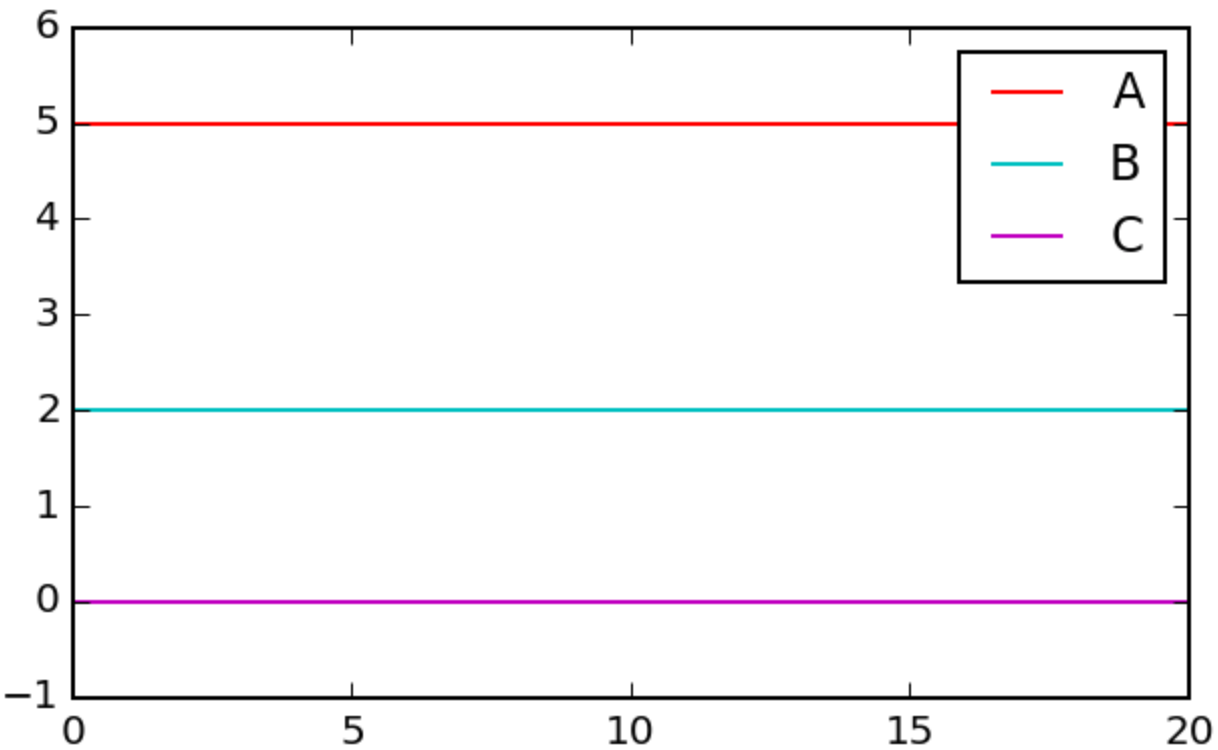
\includegraphics[scale=0.5]{pasted-image-35.png}        
    \end{subfigure}
 
    \caption{Пример простого случая с постоянными значениями}
    \label{fig_parsetree}
\end{figure}

Для таких простых объектов мы можем использовать поточечную разность в качестве функции расстояния, но, если мы сталкиваемся с более сложными графиками, то довольно трудно оценить качество работы такой функции.
Рассмотрим другой пример.
На нём также представлены графики трёх функции.
Но в отличии от предыдущего случая, при использовании функции поточечной разницы для нахождения ближайшего графика к объекту X, мы получим объект Z.
Мы можем заметить, что у графиков X и Y присутствует период и для нас они более похожи между собой, чем Z в качестве прямой.

\begin{figure}[ht]
	\centering
    \begin{subfigure}[b]{1\textwidth}
    \centering
        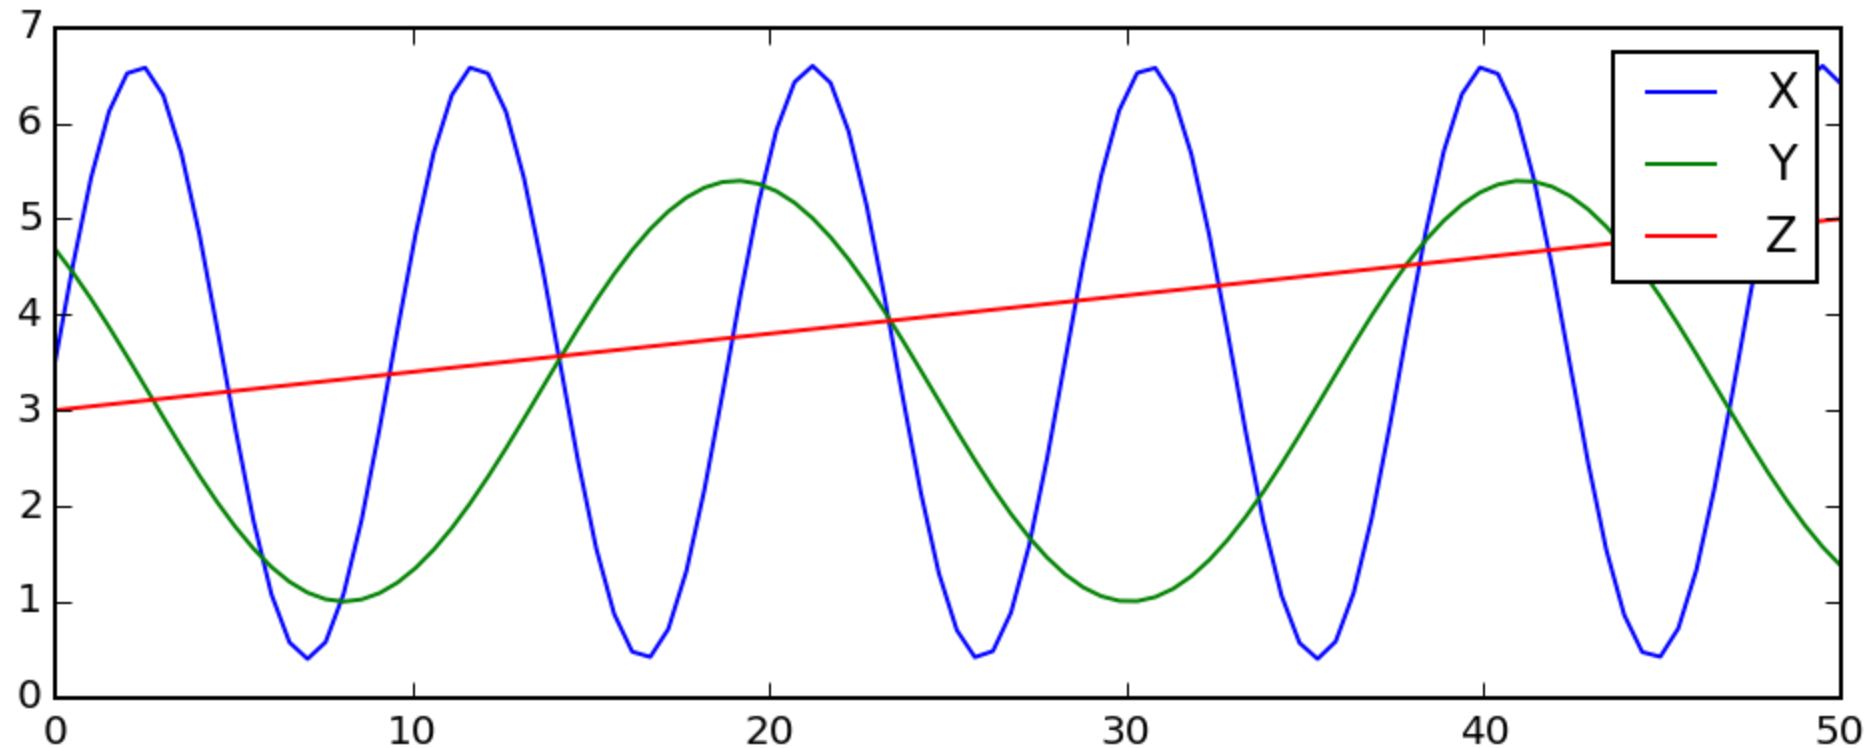
\includegraphics[scale=0.45]{pasted-image-39.png}        
    \end{subfigure}
 
    \caption{Более сложные модели графиков для сравнения}
    \label{fig_parsetree}
\end{figure}

Поточнечная разность как функция расстояния никак не учитывает смещение графиков по оси X, если бы мы перед расчётом разницы выравнивали графики между собой наилучшим способом, то мы бы решили эту проблему.
Одним из известных алгоритмов, пытающихся решить проблему выравнивания и поиска расстояния между двумя графиками, является метод под названием Dynamic Time Warping или DTW.
Его интерфейс довольно прост — он принимает на вход значения двух функций и возвращает расстояние между ними. Данный алгоритм впервые был применён в задачах, связанных с распознаванием речи, сейчас же он используется в различных сферах.

Алгоритм, реализующий DTW, является классической задачей динамического программирования.
Пусть  $Q = \left( q_1, q_2, \dots, q_n \right)$ и $S = \left( s_1, s_2, \dots, s_m \right)$ значения двух функций, переданные нам в качестве входных данных.
Определим вспомогательную матрицу $D$ размером $n$ на $m$.
Зададим начальное значение $D[1, 1] = d(q_1, s_1)$, где $d$ является функцией Евклидового расстояния или любой другой функции расстояния.
Далее остальные ячейки заполняются с помощью правила:

$$D[i, j] = min(D[i, j - 1], D[i - 1, j - 1], D[i - 1, j]) + d(q_i, s_j)$$

\begin{figure}[ht]
	\centering
    \begin{subfigure}[b]{1\textwidth}
    \centering
        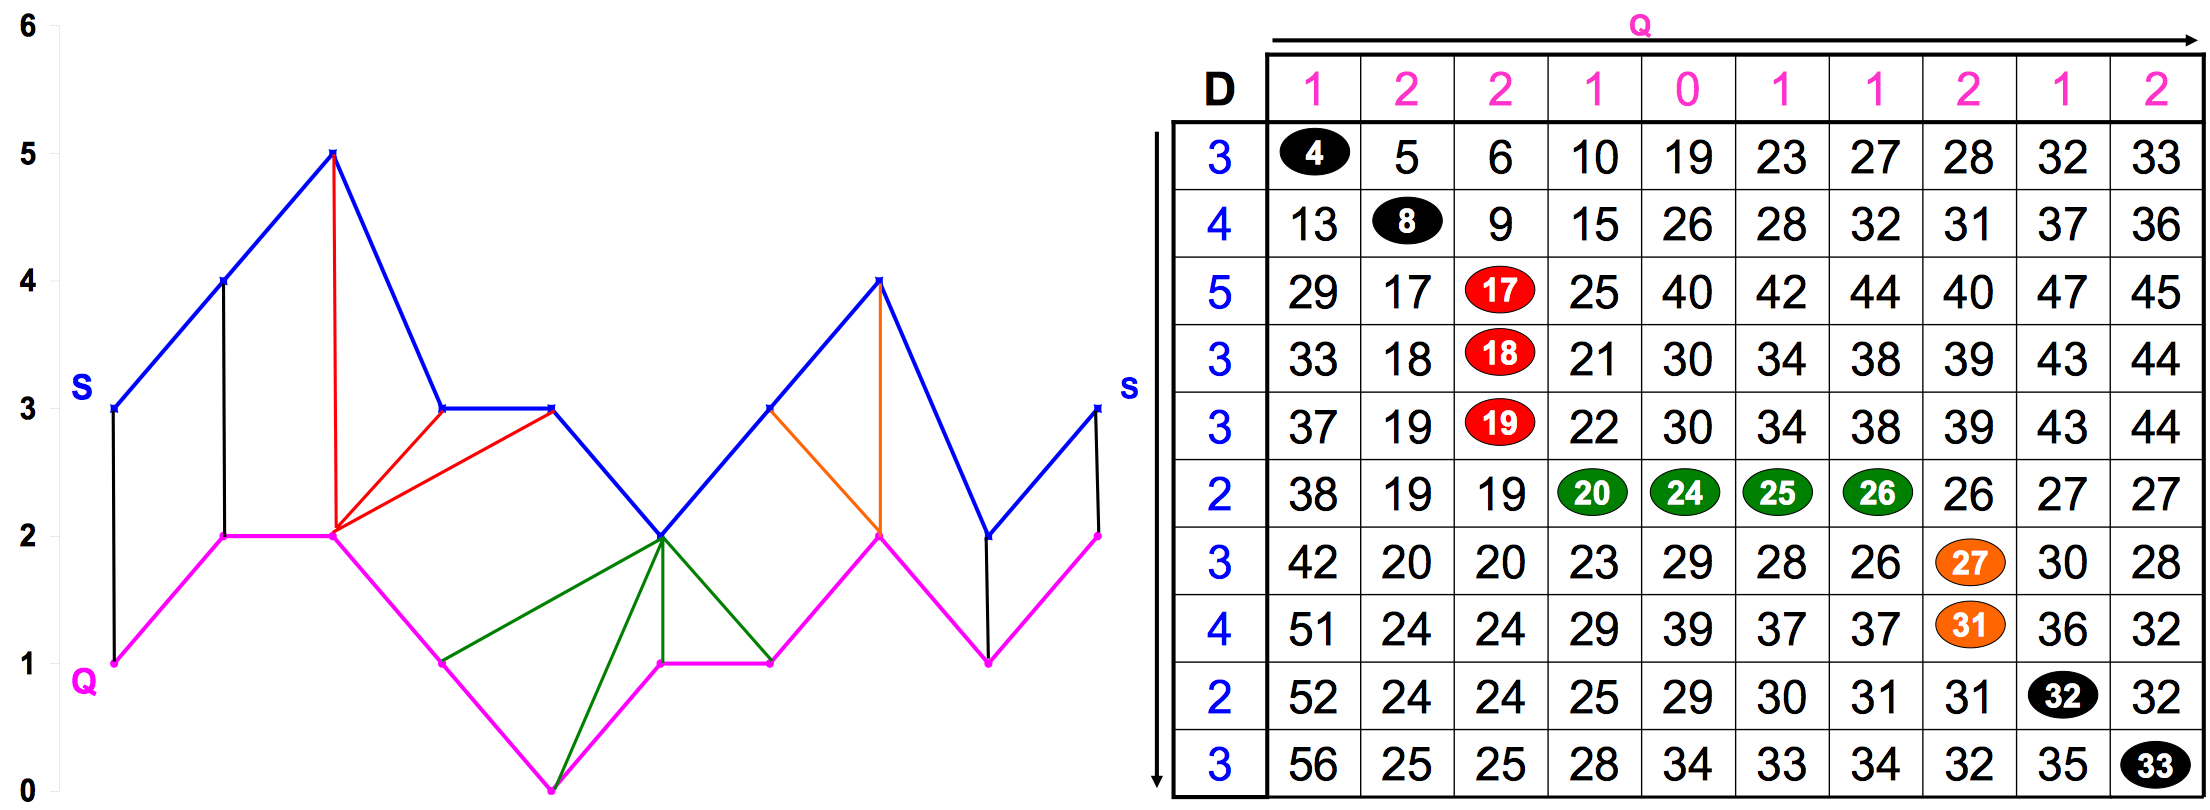
\includegraphics[scale=0.40]{pasted-image-41.png}        
    \end{subfigure}
 
    \caption{Демонстрация работы алгоритма DTW}
    \label{fig_parsetree}
\end{figure}

Конечное расстояние между двумя объектами будет находится в  нижней правой ячейке $D[n, m]$. Стоит заметить что существует модификация данного алгоритма использующее дополнительное численное ограничение $W$ на матрицу. Данное ограничение позволяет не заполнять пути отстающие от диагонали матрицы $D$ более чем на $W$ ячеек, что существенно ускоряет работу алгоритма. Также нетрудно увидеть что сложность алгоритма DTW составляет $O(n m)$, где $n$ и $m$ количество значений каждой функции. Такая сложность связана с необходимостью заполнения матрицы размера $n$ на $m$. 

Итак, мы смогли подобрать функцию расстояния между несколькими сигналами, далее мы ей воспользуемся для создания первого слоя классификаторов реализующих метод K ближайших соседей.

\section{Метрическая классификация, первичный вектор оценок}

Каждый объект, являющийся файлом формата .doc, мы представили набором функций отображающих зависимость между номером определённой операции и временем выполнения этой операции. После перевода сырых данных, представленные утилитой PROCMON, удалось извлеч 24 различных операции: 

\begin{itemize}
\item ‘QueryNameInformationFile'
\item 'SetAllocationInformationFile'
\item 'QueryOpen'
\item 'QueryStandardInformationFile'
\item 'LockFile'
\item 'QueryEaInformationFile'
\item 'SetBasicInformationFile'
\item 'QueryStreamInformationFile'
\item 'QueryBasicInformationFile'
\item 'Thread Create'
\item 'SetEndOfFileInformationFile'
\item 'QueryDirectory'
\item 'Process Profiling'
\item 'FileSystemControl'
\item 'Thread Exit'
\item 'CreateFileMapping'
\item 'Load Image'
\item 'UnlockFileSingle'
\item 'ReadFile'
\item 'WriteFile'
\item 'CloseFile'
\item 'QueryAttributeTagFile'
\item 'CreateFile'
\item 'Process Start’ 
\end{itemize}

Перед тем как начинать работать с графиками, построенными по длительностям собранных операций, нам нужно произвести отбор графиков, точно неподходящих нам. Неподходящими графиками мы будем считать те, которые априори не могут повлиять на конечный результат. Это может быть, например, график с операциями, всегда выполняющихся за время равное 0. Также мы хотим выравнивать по длине графики, построенные по одному типу операций, между всеми объектами. Это нужно для избежания искусственного преимущества одного класса перед другим. Так как явным признаком заражения может являться количество точек в области определения функции, потому что процесс, в котором эксплуатируется какая-либо уязвимость, довольно часто завершается аварийно. 

После такого этапа фильтрации и выравнивания у нас остаётся 14 операций:

\begin{itemize}
\item ‘QueryNameInformationFile'
\item 'SetAllocationInformationFile'
\item 'QueryOpen'
\item 'QueryStandardInformationFile'
\item 'LockFile'
\item 'QueryBasicInformationFile'
\item 'SetEndOfFileInformationFile'
\item 'QueryDirectory'
\item 'CreateFileMapping'
\item 'UnlockFileSingle'
\item 'ReadFile'
\item 'WriteFile'
\item 'CloseFile'
\item ‘CreateFile’
\end{itemize}

 ( Описать для каждого признака почему мы его отфильтровали, разделить на группы по причине. Описать процесс отсечения операций с конца графика. )

Для создания и проверки качества модели, нам необходимо разделить исходную выборку на две части: обучающую и тестовую. Далее будем обучать наш метод на одной выборке и получать результаты для оценки на второй. Как и говорилось ранее, обучать мы будем метод одного ближайщего соседа. Весь алгоритм создания классификатора можно свести к следующим действиям: на этапе обучения мы просто запоминаем выборку, переданную нам, а во время предсказания меток для новых объектов мы с помощью ранее описанного алгоритма DTW находим ближайший график, возвращая его метку класса в качестве ответа.

\begin{figure}[ht]
	\centering
    \begin{subfigure}[b]{0.45\textwidth}
    \centering
        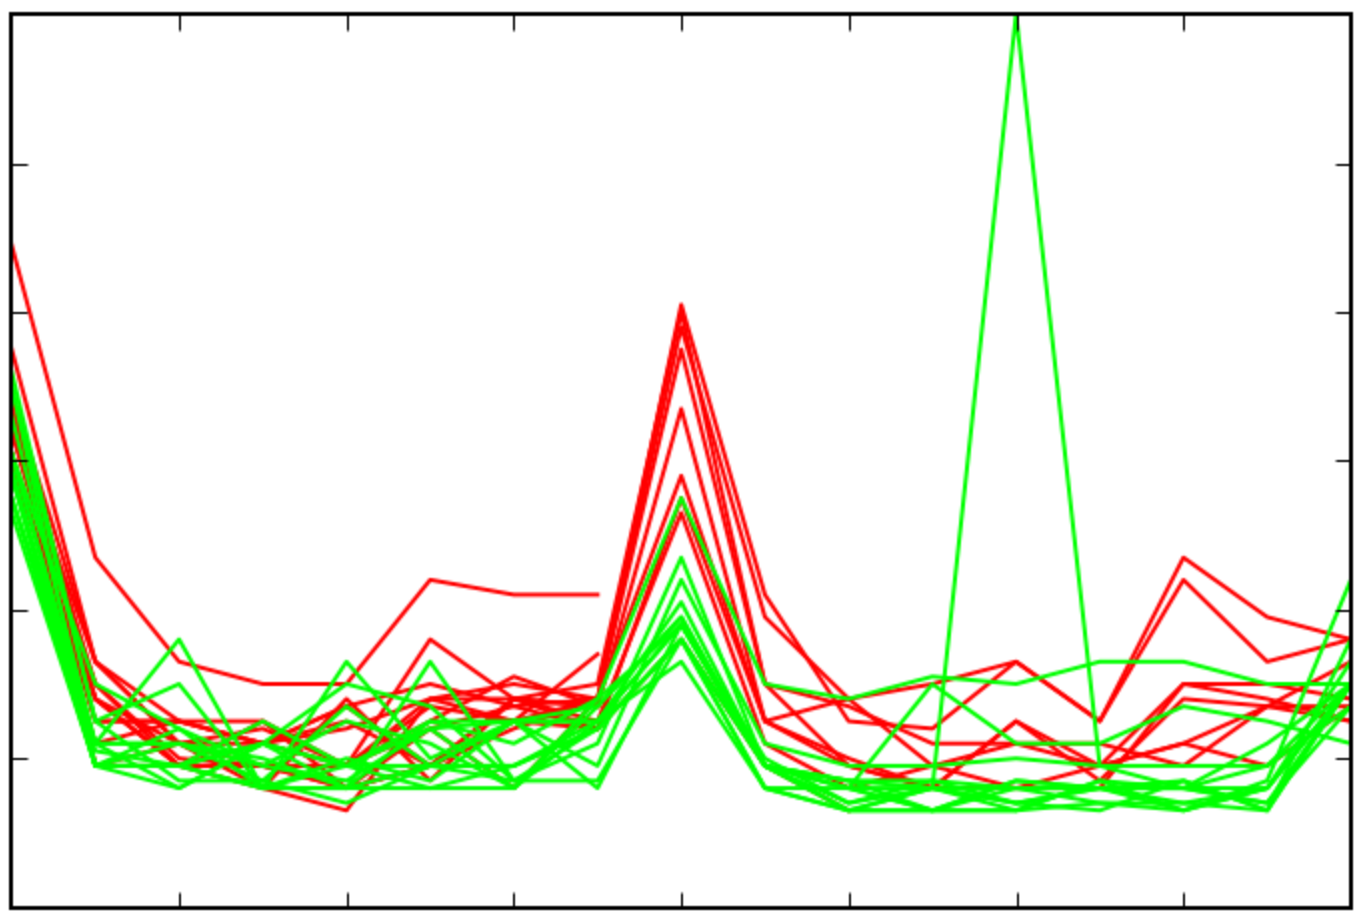
\includegraphics[scale=0.3]{pasted-image-43.png}
        \caption{}
    \end{subfigure}
 	\begin{subfigure}[b]{0.45\textwidth}
    \centering
        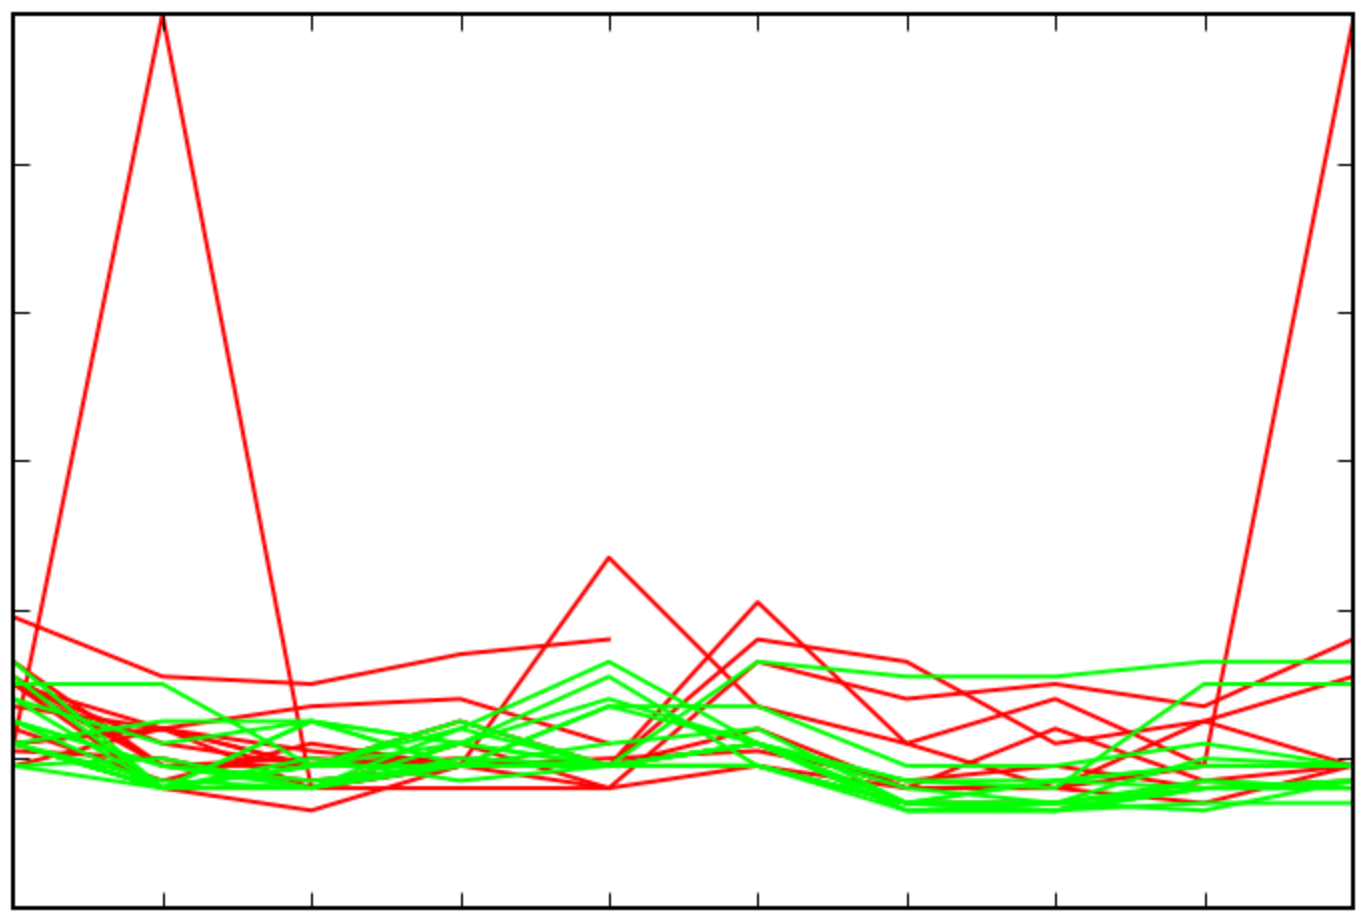
\includegraphics[scale=0.3]{pasted-image-45.png}
        \caption{}
    \end{subfigure}
    \caption{Визуализация нескольких типов сигналов; различным цветом обозначен тип файлов (вредоносные -- красным, безопасные -- зелёным)}
    \label{fig_parsetree}
\end{figure}

Так как размер отфильтрованного набора графиков операций равен 14, то в итоге на каждый объект из тестовой выборки мы получим вектор оценок, состоящий из 14 элементов, каждый элемент которого будет принадлежать множеству $\{0, 1\}$. То есть мы независимо предсказали метку класса по каждому типу операций. По каждому такому вектору нам необходимо вернуть окончательное решение, представляющее итоговую метку исследуемого объекта. Один из самых простых способов отображения вектора меток класса в итоговую метку это взятие большинства, но данный метод никак не учитывает качество работы каждого классификатора. Часто на практике для таких целей используют иной подход: мы можем рассматривать каждый вектор из 14 элементов как входные данные для другого классификатора. В таком случае первый слой классификаторов мы будем называть базовыми классификаторами, а алгоритм, формирующий итоговую оценку, мета-классификатором.

\section{Объединение оценок}

Если посмотреть на вектора оценок, составленных работой базовых алгоритмов, то мы можем увидеть уже знакомый вид матрицы объект-признак, где каждый элемент строки принадлежит отрезку $[0 \dots 1]$.

В итоге наш итоговый классификатор приобретёт многослойный вид. На первом слое находится набор из 14 моделей одного ближайшего соседа с метрикой DTW, пытающихся передать сигнал непосредственно из формальных признаков объекта.
В качестве мета-алгоритма мы будем использовать линейную модель для конечного объединения оценок в итоговую метку класса.
На вход линейной модели будет передан набор векторов из оценок, полученных базовыми алгоритмами.
Такой набор можно аналогично представить как матрицу объект-признак.
Данный многослойный способ построения классификаторов много раз показывал себя с лучшей стороны в мировой практике.

\bgroup
\def\arraystretch{1.5}%  1 is the default, change whatever you need
\begin{table}[ht]
\caption{Оценки базовых алгоритмов, полученных по отобранным сигналам}
\label{tab_weight}
\centering
    \begin{tabular}{|c|c|c|c|c|c|c|c|c|c|c|c|c|c|c|}
    \hline Вид файла & \multicolumn{14}{c|}{Результаты работы базовых алгоритмов} \\
	\hline $G_0$ & 0 & 1 & 0 & 0 & 0 & 0 & 1 & 0 & 0 & 0 & 0 & 1 & 0 & 0 \\
	\hline $G_1$ & 0 & 1 & 0 & 0 & 0 & 0 & 0 & 0 & 1 & 0 & 0 & 0 & 0 & 0 \\
	\hline $B_0$ & 1 & 1 & 1 & 1 & 1 & 1 & 1 & 1 & 1 & 1 & 1 & 1 & 1 & 1 \\
	\hline $B_1$ & 1 & 0 & 0 & 1 & 1 & 1 & 0 & 0 & 1 & 0 & 1 & 0 & 1 & 1 \\

	\hline
    \end{tabular}
\end{table}
\egroup

Единица в ячееке таблицы означает, что для соответствующего файла и типа сигнала ближайшим соседом оказался вредоносный объект.
Если вспомнить, что каждый базовый алгоритм, возвращающий значение в каждой строчке матрицы, строится по отдельной операции, то итоговая линейная модель примет вид взвешенного голосованиями между исходным набором операций. Если по какой-то операции был построен плохой классификатор, часто возвращающий неправильную метку, то во время обучения объединяющей модели такой классификатор получит маленький или вовсе нулевой вес.

\section{Оценка качества итоговой классификации}

Для оценки качества классификации данной конструкции мы разделим исходную выборку объектов на три множества: A, B и C. Используя выборку A, мы будем обучать базовые алгоритмы одного ближайшего соседа, затем предсказав для выборок B и C метки классов по каждому из 14 классификаторов. Таким образом мы получим набор из промежуточных векторов, представляющих матрицу объект-признак. Как последний этап создания классификатора, мы обучим линейный мета-алгоритм на выборке B и предскажем метки классов для объектов из выборки C. Получив качество предсказания выборки C, мы можем поменять между собой выборки B и C и проделать все шаги повторно, получив новый вариант оценок качества. Таким образом, меняя выборки для обучения каждого из слоёв классификаторов, мы сможем получить 6 варинтов оценок, которые стоит усреднить для борьбы с шумом. На каждом этапе построения моделей важно делать обучение на непересекающихся выборках, иначе измеренное качество может получится смещённым.

\bgroup
\def\arraystretch{1.5}%  1 is the default, change whatever you need
\begin{table}[ht]
\caption{Оценки базовых алгоритмов}
\label{tab_weight}
\centering
    \begin{tabular}{|c|c|c|c|}
	\hline Варианты разбиений & Точность & Полнота & F-мера \\
	\hline 1 & 1 & 0.59 & 0.74 \\
	\hline 2 & 1 & 1 & 1 \\
	\hline 3 & 1 & 0.80 & 0.88 \\
	\hline 4 & 0.71 & 1 & 0.83 \\
	\hline 5 & 1 & 1 & 1 \\
	\hline 6 & 1 & 0.8 & 0.88 \\
	\hline Итоговая оценка & 0.95 & 0.86 & 0.89 \\
	\hline
    \end{tabular}
\end{table}
\egroup

Получив усреднённые оценки, мы увидим, что точность нашего метода близка к единице. На практике это означает, что почти все вредоносные объекты будут верно классифицированы. Чуть меньше оказалась величина полноты равна 0.86. Это говорит нам о том, что, во время использования алгоритма, примерно 14\% безвредных объектов будут распознаны как вредоносные.